\newcommand{\chapter}[2][]{
	\newcommand{\chapname}{#2}
	\begin{flushleft}
		\begin{minipage}[t]{\linewidth}
			
\includegraphics[height=1cm]{hdht-logo.png}
			\hspace{0pt}	
			\sffamily\bfseries\large Bài  2.
			\begin{flushleft}
				\huge\bfseries #1
			\end{flushleft}
		\end{minipage}
	\end{flushleft}
	\vspace{1cm}
	\normalfont\normalsize
}
\chapter[Sai số khi đo các đại lượng vật lí - Các quy tắc an toàn trong phòng thực hành vật lí]{Sai số khi đo các đại lượng vật lí - Các quy tắc an toàn trong phòng thực hành vật lí}
\section{Lý thuyết}
	\subsection{Phép đo các đại lượng vật lí - Hệ SI}
\subsubsection{Phép đo các đại lượng vật lí}
Phép đo một đại lượng vật lí là phép so sánh nó với đại lượng cùng loại được quy ước làm đơn vị.

Phép so sánh trực tiếp nhờ dụng cụ đo gọi là phép đo trực tiếp.

Phép xác định một đại lượng vật lí thông qua một công thức liên hệ với các đại lượng đo trực tiếp, gọi là \bltext{phép đo gián tiếp}.
\subsubsection{Đơn vị đo}
Một hệ thống các đơn vị đo các đại lượng vật lí được quy định thống nhất áp dụng tại nhiều nước trên thế giới, trong đó có Việt Nam, gọi là hệ SI.
\subsection{Sai số phép đo}
Sai số phép đo bao gồm \bltext{sai số dụng cụ} và \bltext{sai số ngẫu nhiên}.
\subsection{Giá trị trung bình}
Khi đo $n$ lần cùng một đại lượng $A$, ta thu được các giá trị khác nhau: $A_1,\, A_2,\,...,A_n$

Giá trị trung bình khi đo nhiều lần một đại lượng $A$:$$\bar{A}=\dfrac{A_1+A_2+...+A_{\text{n}}}{n},$$
là giá trị gần đúng nhất với giá trị thực của đại lượng $A$.  
\subsection{Cách xác định sai số của phép đo}
\begin{itemize}
	\item Sai số tuyệt đối ứng với mỗi lần đo:
	$$\Delta A_1=|\bar{A}-A_1|;\,\Delta A_2=|\bar{A}-A_2|;\,\Delta A_3=|\bar{A}-A_3|;...$$
	\item Sai số ngẫu nhiên là sai số tuyệt đối trung bình của $n$ lần đo:
	$$\overline{\Delta A}=\dfrac{\Delta A_1+\Delta A_2+...+\Delta A_{\textrm{n}} }{n}.$$
	\item Sai số dụng cụ $\Delta A'$ có thể lấy bằng nửa hoặc một độ chia nhỏ nhất trên dụng cụ.
	\item Sai số tuyệt đối của phép đo là tổng \bltext{sai số ngẫu nhiên} và \bltext{sai số dụng cụ}:
	$$\Delta A= \overline{\Delta A}+ \Delta A'.$$
\end{itemize}
\subsection{Cách viết kết quả đo}
$$A=\overline{A} \pm \Delta A,$$
trong đó:
\begin{itemize}
	\item $\overline A$ là giá trị trung bình,
	\item $\Delta A$ là sai số tuyệt đối. 
\end{itemize}
\subsection{Sai số tỉ đối}
Sai số tỉ đối $\delta A$ của phép đo là tỉ số giữa \bltext{sai số tuyệt đối} và \bltext{giá trị trung bình} của đại lượng cần đo, tính bằng phần trăm:
$$\delta A=\dfrac{\Delta A}{\overline A}\cdot 100\%.$$
Sai số tỉ đối càng \bltext{nhỏ} thì phép đo càng chính xác.
\subsection{Cách xác định sai số của phép đo gián tiếp}
Sai số của phép đo gián tiếp, được xác định theo các quy tắc:
\begin{itemize}
	\item Sai số tuyệt đối của một tổng hay hiệu thì bằng \bltext{tổng} các sai số tuyệt đối của các số hạng.
	\item Sai số tỉ đối của một tích hay thương thì bằng \bltext{tổng} các sai số tỉ đối của các thừa số. 
\end{itemize}
\subsection{Một số quy định về an toàn trong phòng thực hành vật lí}
\subsubsection{Quy tắc an toàn trong sử dụng các thiết bị điện}
Cần quan sát kĩ các kí hiệu và nhãn thông số trên thiết bị để sử dụng đúng chức năng, đúng yêu cầu kĩ thuật.

Một số kí hiệu trên các thiết bị thí nghiệm:
\begin{center}
	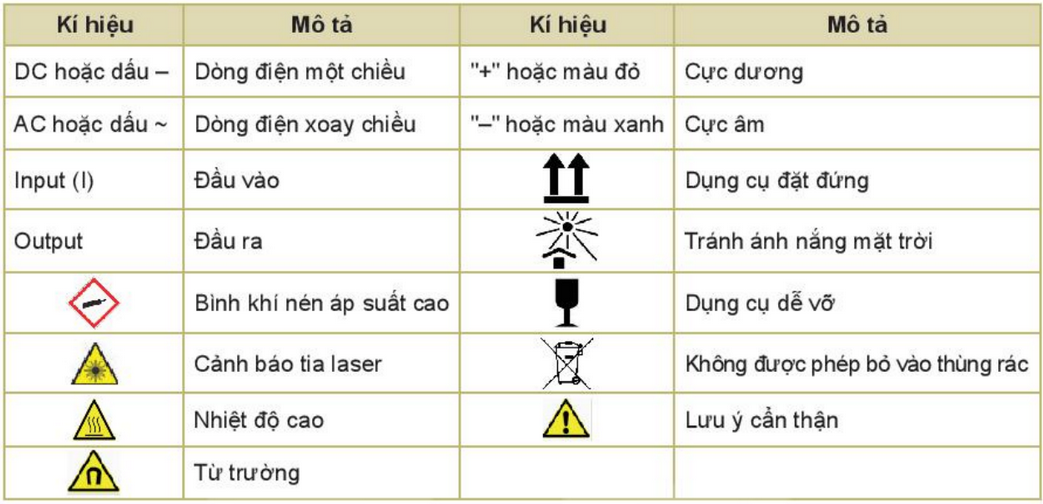
\includegraphics[scale=0.8]{../figs/G10-2-1}
\end{center}
\subsubsection{Quy tắc an toàn sử dụng các thiết bị nhiệt và thủy tinh}
Các thiết bị đun nóng có thể gây cháy hoặc nứt, vỡ các dụng cụ bằng thuỷ tinh.
\subsubsection{Quy tắc an toàn sử dụng các thiết bị quang học}
Các thiết bị quang học rất dễ bị mốc, xước, nứt, vỡ và dính bụi bẩn, làm ảnh hưởng đến đường truyền tia sáng và sai lệch kết quả thí nghiệm.
\section{Mục tiêu bài học - Ví dụ minh họa}
\begin{dang}{Xác định được sai số tuyệt đối, sai số tỉ đối\\và biểu diễn kết quả đo}
	\viduii{3}{Trong bài thực hành đo gia tốc trọng trường của Trái Đất tại phòng thí nghiệm, một học sinh đo được chiều dài của con lắc đơn $l= (800 \pm 1)$ mm thì chu kì dao động là $T = (1,78 \pm 0,02)$ s. Lấy $\pi$ = 3,14. Biết chu kỳ của con lắc đơn tính theo công thức $T=2\pi \sqrt{l/g}$. Gia tốc trọng trường $g$ của Trái Đất tại phòng thí nghiệm đó là bao nhiêu?
	}
	{	\begin{center}
			\textbf{Hướng dẫn giải}
		\end{center}
		
	Từ công thức: $$T=2\pi \sqrt{\dfrac{l}{g}} \Rightarrow g=\dfrac{4\pi^2l}{T^2}.$$ 	
	
	Giá trị trung bình của gia tốc trọng trường: 	
	$$\overline{g}=\dfrac{4\pi^2l}{T^2}=\dfrac{4\pi^2\cdot 3,14^2\cdot 0,8 \,\text{m}}{\left( 1,78 \,\text{s}\right) ^2}=9,96 \,\text{m/s}^2.$$
	
	Sai số tuyệt đối của gia tốc trọng trường:
	$$\dfrac{\Delta g}{\overline g}= \dfrac{\Delta l}{\overline l}+ 2\dfrac{\Delta T}{\overline T}=\dfrac{1\, \text{mm}}{800\, \text{mm}}+2\dfrac{0,02\, \text{s}}{1,78\, \text{s}}=0,024. $$
	
	
	$$\Rightarrow \Delta g= 0,024\cdot \overline g= 0,24 \text{m/s}^2.$$
	
	
	Vậy gia tốc trọng trường của Trái Đất tại phòng thí nghiệm đó là:
	$$g={\overline g } + \Delta g =9,96 \pm 0,24\, \text{m/s}^2.$$
	}
	\viduii{3}{Một học sinh dùng cân và đồng hồ đếm giây để đo độ cứng $k$ của lò xo. Dùng cân để cân vật nặng thu được kết quả khối lượng $m = 100 \,\text{g}$ với sai số tỉ đối là $2\%$. Gắn vật vào lò xo và kích thích cho con lắc dao động rồi dùng đồng hồ đếm giây đo thời gian của một dao động cho kết quả $T = 2\,\text{s}$ với sai số tỉ đối là $1\%$. Biết chu kỳ của con lắc lò xo tính theo công thức $T=2\pi \sqrt{m/k}$. Sai số tỉ đối của phép đo độ cứng của lò xo là bao nhiêu?
	}
	{	\begin{center}
			\textbf{Hướng dẫn giải}
		\end{center}
		
		Từ công thức: $$T=2\pi \sqrt{\dfrac{m}{k}} \Rightarrow k=\dfrac{4\pi^2m}{T^2}.$$	
		
		Sai số tỉ đối của độ cứng lò xo: 	
		$$\dfrac{\Delta k}{\overline k}= \dfrac{\Delta m}{\overline m}+ 2\dfrac{\Delta T}{\overline T}= 2\%+2\cdot 1\%= 4\%.$$
		
		Vậy sai số tỉ đối của phép đo độ cứng của lò xo là $4\%.$
	}
\end{dang}

\begin{dang}{Vận dụng được các quy tắc an toàn trong phòng thực hành vật lí}
	\viduii{2}{Hãy nêu quy tắc an toàn trong việc sử dụng các thiết bị sau:
		\begin{enumerate}
			\item Phích cắm điện;
			\item Dây điện;
			\item Nguồn tia LASER;
			\item Đèn cồn.
		\end{enumerate}
	}
	{	\begin{center}
			\textbf{Hướng dẫn giải}
		\end{center}
		
		\begin{enumerate}
			\item Phích cắm điện: Không chạm tay vào vị trí tiếp xúc giữa phích cắm và ổ điện, không cắm điện khi tay ướt.
			\item Dây điện: Không sử dụng dây điện cũ, không đấu nối dây điện thiếu an toàn.
			\item Nguồn tia LASER: Không đặt mắt trực tiếp trên đường truyền của tia LASER, không chiếu tia LASER vào người khác;
			\item Đèn cồn: Không bỏ đi nơi khác khi đang đun bằng đèn cồn, hơ lửa đều để ống nghiệm giãn nở đều.
		\end{enumerate}
	}
	\viduii{2}{Hãy cho biết các dụng cụ đo sau có chức năng gì và cách nối chúng vào mạch điện:
		\begin{enumerate}
			\item Ampe kế;
			\item Vôn kế;
			\item Đồng hồ đo điện đa năng.
		\end{enumerate}
	}
	{\begin{center}
			\textbf{Hướng dẫn giải}
		\end{center}
		
		\begin{enumerate}
			\item Ampe kế: Dùng để đo cường độ dòng điện, nối tiếp với đoạn mạch cần đo;
			\item Vôn kế: Dùng để đo hiệu điện thế, mắc song song với đoạn mạch cần đo;
			\item Đồng hồ đo điện đa năng: Dùng để đo hiệu điện thế, cường độ dòng điện và điện trở, cần vặn núm xoay vào thang đo phù hợp trước khi tiến hành đo.
		\end{enumerate}
	}
\end{dang}